\chapter{Background}
\label{chapter:background}

% 1. how the literature was collected (describe it pragmatically)
%
% 2. literature review (summary, analysis, and comparisons)
%
%   A literature review should answer:
%
%     * What do we already know about the topic?
%     * What do you have to say critically about what is already known?
%     * Has anyone else done anything exactly the same?
%     * Has anyone else done anything that is related?
%     * Where does your work fit in with what is done before?
%     * Why is your research worth doing in the light of what has
%       already been done?
%
%   A literature review should be a dialogic rather than a mere
%   replication of other peoples writing. Should not be a laundry
%   list of previous studies.
%
%   Be focused and critical. Include an incisive critique that will help your
%   peers see the world differently.
%
% 3. introduction to terms as folksonomy, tagging, geotagging, etc
%
% 4. paragraph or two about my subject related to popular literature
%    (search Amazon or Library of Congress and say something like: there
%    were X books about this subject, the first was published in 2001
%    but the majority of books were published the last two years, and
%    maybe show a graph)

\section{Literature Search}

Before a literature search was conducted we did some preliminary thinking
about
\begin{inparaenum}[(i)]
  \item the focus of our topic to get more precise results, and
  \item what literature databases would yield sufficient and accurate
    findings.
\end{inparaenum}
Based on these concerns we settled on the literature indexes laid out in
\tableref{literature.databases} and used the following keywords%
\sidenote{
  With varying use of modifiers (i.e. AND) or quotations to find exact phrases
}
for search:

\begin{description}
  \item[social navigation] is the concept of our main topic.
  \item[collaborative filtering] is often used to realize our main topic.
  \item[recommender system] can be an application of our main topic.
  \item[tagging] can be related to our topic depending on use.
\end{description}

\begin{table}
  \centering
  \caption{Literature Databases}
  \label{table:literature.databases}

  \begin{tabular}{p{20pc}l}

    \toprule
    Name & Type \\
    \midrule

    ACM Digital Library &
    Full-text \\

    The Collection of Computer Science Bibliographies &
    Bibliography \\

    Inspec Online &
    Reference \\

    HCI Bibliography &
    Bibliography \\

  \end{tabular}
\end{table}

In addition to keyword based search we also conducted citation searches on the
articles that in our opinion seemed to be the most important in the field.
The articles that we found relevant during our literature search phase was
collected and studied. During this process we eliminated articles by the same
authors where similar topics and implementations were discussed and focused on
either the most recent or the most representative article.

First we'll briefly discuss navigation and sociality both in general terms
and relating to the web. Then we'll concentrate on these two topics together
by looking at the research where social navigation is used
consciously as a concept. By this we mean the research where either social
navigation is defined, redefined or problems relating to the concept is
discussed with a basis in such definitions.
After our main survey of social navigation research we'll look at topics
which we believe can be included in the discussion of social navigation or are
closely related.

Some of the research that has been conducted in the space of
social navigation and related areas does not share our focus on the Web.
We still found much such research interesting in spite of their attention to
generalized problems or specific problems in other fields than the Web.

\section{Navigation}
% Try to cite some classic work. First navigation systems

Navigation was traditionally associated with controlling a weasel at sea to
a given destination.%
\sidenote{
  \emph{Navigate} is in fact derived from the two Latin words \emph{navis}
  meaning ``ship'' and \emph{agere} meaning ``to drive''.
  \citep[p.~756]{anderson97}
}
Since then it's been used to describe behavior related to safely finding ones
way whether one is driving a car, flying a plane or walking on foot. Maps
(a graphical representation of the medium one are navigating in)
and compass (a tool for connecting graphical maps to the physical world)
are often used as aids in this way finding. When used in context of
computer systems navigation is essentially a metaphor of our usage of the
word in our physical world. Trough computer systems we present users with a
conceptual space in which they can navigate \citep[p.~189]{whiteside85}.

\subsection{Navigation on the Web}

Navigation is important on the Web. Without a way to efficiently and safely
navigate one is in the danger of becoming lost. This problem was evident even
before the Web was invented:
\begin{citequote}[p.~38]{conklin87}
  Hypertext offers more degrees of freedom, more dimensions in which one
  can move, and hence a greater potential for the user
  to become lost or disoriented.
\end{citequote}

\citet{jones96} studied the navigational support provided by the Web's first
browsers:
\begin{inparaenum}[(i)]
  \item loading of page by entering it's location,
  \item loading a bookmarked page,
  \item loading a page by using a hyperlink on the current page,
  \item recall previously visited pages with forward and backward buttons,
  \item recall a previously visited page by locating it in a history list, and
  \item reloading the current page.
\end{inparaenum}
While modern web browsers support more forms of navigation%
\oddsidenote{
  These early browsers' history lists were not remembered between sessions. In
  addition we're seeing browsers as Flock (available at
  \url{http://flock.com}) with new methods of navigation integrated and also
  an abundance of plugins and extensions for the main stream browsers that
  enable new possibilities for navigation.
}
than the earliest applications we're not concerned with those here.
We're only interested in the navigation which are conducted within the main
browser window (where web pages are rendered) enabled by following hyperlinks.

\section{Sociality}

In the Oxford English Dictionary, second edition \citep[p.~905]{simpson89}
the adjective \emph{social} is defined as:

\begin{quote}
  Capable of being associated or united \emph{to} others.
\end{quote}

Discussion about explicit social matters is left for scholars of the social
sciences. We've therefore briefly introduced the term and are more concerned
with situations where it's related to computer systems, and most importantly:
the Web.

\subsection{Sociality on the Web}
% Discuss sociality on the web. Maybe a good place for a Web 2.0 discussion.

Sociality has become an integral part of our modern age version of the Web.
\citeauthor{bernerslee07}, seen by many as the inventor of the Web,
recently discussed the evolution from the Net (III: International
Information Infrastructure), trough the Web (WWW: World Wide Web),
to what he calls \emph{the Graph} (GGG: Giant Global Graph) in a
blog post \citeyearpar{bernerslee07}. The Graph is synonymous with the
\emph{Semantic Web}%
\sidenote[-8\onelineskip]{
  The Semantic Web is a web where data and information can be meaningful
  to computers and not just humans \citep{bernerslee01}. Although this idea
  was introduced by \citeauthor{bernerslee07} in 1994 it remains largely
  unrealized to this day \citep[p.~96]{shadbolt06}.
}
and he describe it in relation to
current trends of sociality on the Web:
\begin{citequote}{bernerslee07}
  It's not the Social Network \emph{Sites} that are interesting--it is the
  Social Network itself. The Social Graph.
\end{citequote}

In other terms this means that social relationships on the Web have become so
important that they're more interesting themselves than the pages that
represents them. While it would be very interesting to look at how
\emph{social navigation} (to be discussed shortly) can be enabled between
different web pages and web services%
\sidenote[-10\onelineskip]{
  Examples of social navigation between different web sites can be seen in
  many of Facebook's (discussed in \sectionref{analysis.facebook}) third party
  applications, Google's similar \emph{OpenSocial} initiative (Available at:
  \url{http://code.google.com/apis/opensocial/}), and various \emph{mashups}
  (to be discussed shortly) between open web services.
}, we're leaving it out of our research
due to the time constraints a master thesis inherits.

\subsubsection{Web 2.0}
% tie in definition from oreilly in introduction chapter.
% cite web 2.0 general papers
% cite weiss05 paper, collective intelligence
% introduce mashups (maybe sub-sub-section) as it's been used in side-note above.
% self sufficient user base
% need early adopters, not immediate benefit before the user base is sufficient
% large. term for this, can't remember the name

\section{Social Navigation}
\label{section:background.social.navigation}
Drawing on the previous explanation of navigation and definition of social, we
can combine the two terms. Social navigation then means going from one point
to another in a medium with other people.

Social navigation as a term was introduced in a short article by
\citet{dourish94} where they discussed three types of navigational mechanisms,
spatial, semantic, and social, which they argue can be separated even though
there is evidence of situations where the different mechanisms are combined.
In their description of the social type they coined the term
\emph{social navigation}:

\begin{citequote}[p.~1]{dourish94}
  When navigable information systems are extended to support collaborative
  activity, a third model of navigation arises. This is \emph{social}
  navigation. In social navigation, movement from one item to another is
  provoked as an artifact of the activity of another or a group of others.
\end{citequote}

\citeauthor{dourish94} exemplifies two cases where neither location
(spatial) nor content (semantic) is used for exploration--the social model
is used on it's own. Based on these two experiences \citeauthor{dourish94}
argues that we possibly need to move away from spatial models of navigation
and rather focus on designing explicitly with semantic and social navigational
techniques.

\citeauthor{dieberger97} highlights an important aspect for making interaction
on the Web smoother. With an ``awareness of the presence of
other users'' \citeyearpar[p.~812]{dieberger97} one can give an indication of
what parts of a web page that is of high demand and possibly identify the
users accessing them.

\citet[p.~39]{dieberger00b} include the properties of \emph{personalization}
and \emph{dynamism} into their understanding of what social navigation is.
Social navigation is not pre-planned, but grown dynamically in an organic
fashion. This distinction is shown by the example of walking down a road in a
city versus walking on a forest trail. Personalization means that the
navigation advice is given to the receiver in a fashion that suits him.
Related to dynamism is social navigation's temporal nature.
\citet[p.~39]{dieberger00b} shows this with the analogy of a forest trail
which will vanish if it's not used. This idea was envisioned for computer-like
systems by \citeauthor{bush45} over half a decade ago in that
  ``trails that are not frequently followed are prone to fade, items are
  not fully permanent'' \citeyearpar[p.~106]{bush45}.

\citet{svensson05} argues that while social navigation is plentiful in
our everyday world it's not implied that it's a good idea to implement
computer based systems with this perspective in mind. Instead of creating
translations from our physical world to our virtual world
they explain that one instead have to
  ``make information spaces afford social interactions and accumulate
  social trails'' \citeyearpar[p.~377]{svensson05}.
With \emph{social trails} the authors mean traces left in the system by past
users guiding current users' navigational behavior.

\citeauthor{robins02} on the other hand argues that one can not rely on
technological structures alone when one is using social navigation which
  ``transforms a space on a computer network into a virtual place''
  \citep[par.~50]{robins02}.
During an ethnographic study the author examined social navigation in relation
to the persistent structures found in the physical world during a distance
education programme. She found that these real world structures supported and
afforded social navigation in virtual places.

\subsection{Definition}

The most detailed definition of social navigation to our knowledge was
completed by \citet{svensson03} in his Ph.D. thesis. To understand his
definition we'll have to introduce his wording of the actors in a social
navigation process:

\begin{description}
  \item[Navigator] is ``the person seeking navigational advice''
    \citep[p.~20]{svensson03}.
  \item[Advice provider] is a ``person or artificial agent providing
    navigational advice to a navigator'' \citep[p.~20]{svensson03}.
\end{description}

Social navigation was then defined as:

\begin{citequote}[p.~20]{svensson03}
  navigation that is conceptually understood as driven by the actions from one
  or more advice providers.
\end{citequote}

Firstly, \citeauthor{svensson03} talks about navigation with is ``conceptually
understood'' as driven by these advice providers. As long as the user believes
his navigational choices are driven by advice providers it is social
navigation. Secondly, the actions that the navigator is driven by need not be
only direct advice from a single advice provider, but can also be aggregated
of nature.

\subsection{Fundamental Categorization}
% discuss fundamental groupings of social navigation, explicit, implicit and
% so on

We'll take a look at broader characteristics of social navigation
before we'll continue with a discussion of several technical applications of
social navigation found in secondary academic literature.

\subsubsection{Active, Direct, Passive, and Indirect Social Navigation}

In his classic article \citet{dieberger97} distinguishes between an
\emph{active} and \emph{passive} form of social navigation. This distinction
is grounded in the nature of the exchange of information between the two
parties involved in a social navigation process: the advice
provider--the creator of navigation cues--and the navigator.

\begin{description}
  \item[Active] social navigation finds place when a person either
    deliberately seeks out another and asks for a navigation advice or
    intentionally gives away such navigational advice.
  \item[Passive] social navigation happens when people make available
    navigational aids that later can be used by other people.
\end{description}

\citeauthor{svensson03} groups social navigation in \emph{direct}
and \emph{indirect} forms:

\begin{description}
  \item[Direct] social navigation is where ``communication between navigator
    and advice provider is mutual and two-way''
    \citep[p.~21]{svensson03}.
  \item[Indirect] social navigation occurs when ``communication between
    navigator and advice provider is non-mutual and in one direction''
    \citep[p.~21]{svensson03}.
\end{description}

Despite \citeauthor{svensson03}'s more precise wording active social
navigation is similar to direct social navigation. Both are differentiated
with passive social navigation which is similar to indirect social navigation.
\citeauthor{dieberger97} characterize the relationship between the
navigator and advice provider. \citeauthor{svensson03} on the other hand
describes the nature of the communication between the two parties.

\subsubsection{Explicit and Implicit Advice}

Related to passive or indirect social navigation is the notion
of \emph{explicit} and \emph{implicit} feedback. Though generally used to
describe the form of feedback in so called \emph{recommender systems}%
\sidenote{
  Recommender systems is discussed as an application of
  \emph{collaborative filtering} in 
  \sectionref{background.social.navigation.applied.forms.collaborative.filtering}.
}
\citep[p.~82]{oard98} it can also be used more generally to distinguish how
passive or indirect social navigation is provided by an advice provider.
Collect such advide explicitly means that the advice provider have to use
concious effort to do so. For instance such an advice provider can choose to
share an interesting web site and does so by putting a hyperlink to it on his
web page.

When advice is mediated implicitly the process of doing so are transparent and
unintrusive for the advice provider. Based on the work the advice provider
would have done regardless of the social effects it conveys one can provide
advice to future navigators. An example of such behaviour is recording of
browsing history that can be computationally evaluated to provide advice for
others as we'll return to in
\sectionref{background.social.navigation.applied.forms.interaction.history}.

% directly visible or aggregated and hidden in the interaction history of a
% physical object or place dieberger00b

\subsection{Applied Forms}

Social navigation have been applied in several different forms described in
academic literature. Here we'll describe these various forms of social
navigation on the Web.

\subsubsection{Hyperlink Sharing}

\citet{dieberger97} is particularly concerned with making handling of
\emph{URL}%
\oddsidenote{
  Uniform Resource Locator. URL was formerly an abbreviation of Universal
  Resource Locator.
}
entities transparent for users in different tools related to web browsers and
the operating system itself. Making URLs invisible to users will in his
opinion enable more widespread use of social navigation trough pointer
sharing. Web browsers handles URLs embedded as hyperlinks
transparently so we're not going to elaborate on matters of URL handling in
auxiliary systems here.

Both \cite{dourish94} and \cite{dieberger97} observed social navigation on the
Web when hyperlinks were shared on web pages. Creators of these pages often
had a list of pointers to other web pages they deemed interesting enough to go
trough the trouble of creating such a listing. By doing this they created
an opportunity for navigation based on social factors.

% should this be in the analysis section?
While pointer pages still is in existence it seems that the increasing
use of blogs (see \tablepageref{blog.usage})
have resulted in a new form for sharing interesting web pages,
which often is other blogs. So called \emph{blogrolls} is a way for blog
authors to list other blogs they are reading regularly. They thereby function
``as a navigation tool for readers to find other authors with similar
interests'' \citep[p.~3]{marlow07}. An example of a blogroll can be seen in
\figureref{scrsh.dailykos.blogroll}.

\sidefigure{Blogroll}{%
  Blogroll for Daily Kos,
  retrieved December 5, 2007, from
  \url{http://www.dailykos.com/}.
  \label{figure:scrsh.dailykos.blogroll}
}{%
  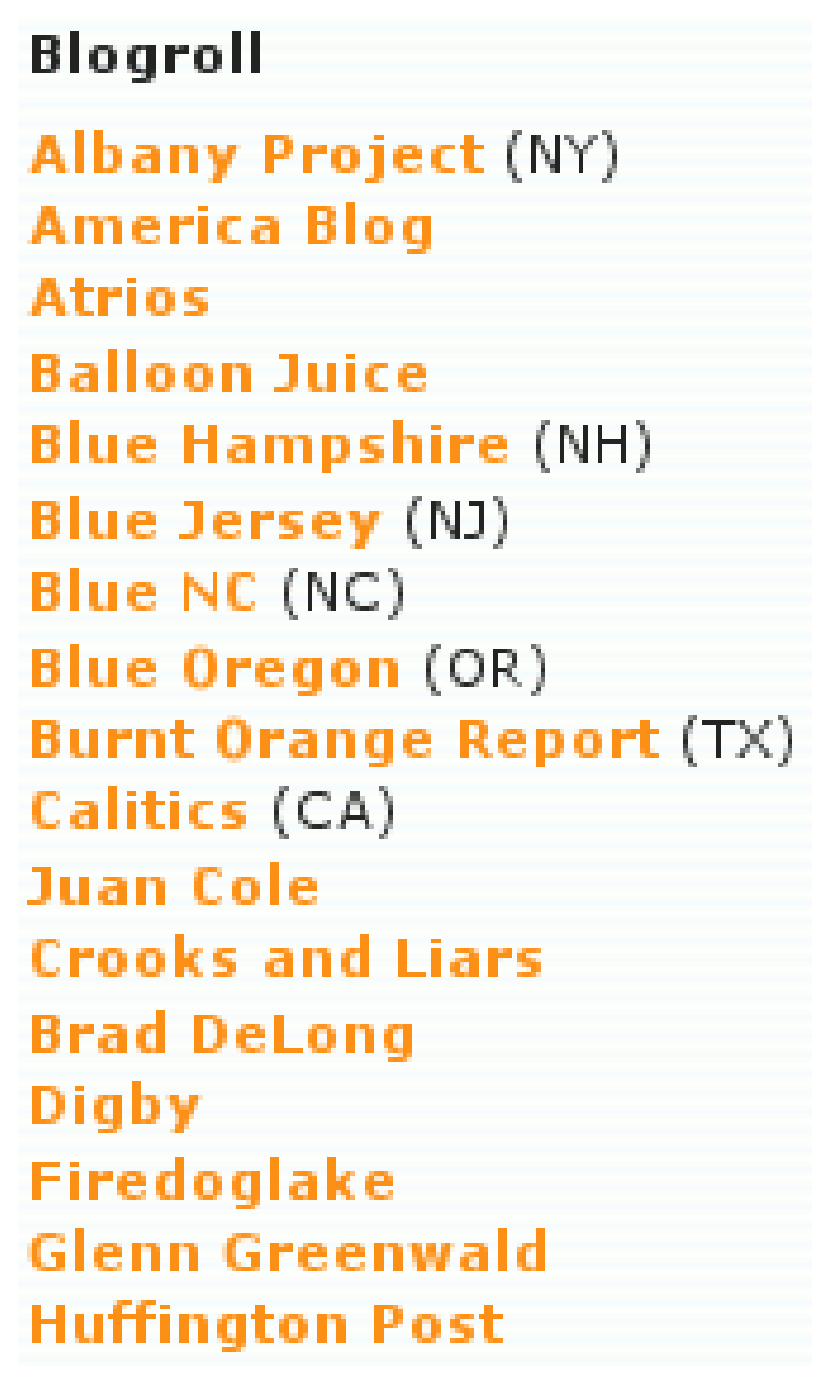
\includegraphics[width=0.9\marginparwidth]{scrsh_dailykos_blogroll}
}

A new phenomena appeared to the mainstream with the introduction of the
\emph{del.icio.us}%
\sidenote{
  % fill in here
}
social bookmarking system. This web page made individual
bookmark collections globally available, making it easy to discover what other
people takes notice of.
%cite, discuss further, lead in to next section.

As \citet[p.~806]{dieberger97} argues the Web's growth, even at it's modest
size of 1997 compared to it's staggering size over 10 years later, have
implications on how easily it is to locate information. By creating pointer
pages, and now socially shared bookmarking services, users are imposing a
structure on the web. By navigating these kinds of interlinked hyperlink
collections it could be that users are getting access to more related and
higher quality information. Sharing a hyperlink, either on you web page or
trough a bookmarking service, requires a conscious effort. One would believe
that people only choose to do so for information they find interesting.

\subsubsection{Item Annotation}
% tagging
% articles with tagging in context of social navigation
% lot of more discussion of tagging and mostly related to organizing
% principles and folksonomy

In addition to being a modern form of pointer pages, social bookmarking
introduced a new way to annotate items. By applying textual key words to
bookmarks--and later other types of content--users were able to browse such
collections in new ways. These key words have been popularized as \emph{tags}
and the act of applying them is called \emph{tagging}. Tagging enables a user
driven ontology%
\evensidenote{
  An ontology has been defined as
    ``a specification of a representational vocabulary for a shared
    domain of discourse--definitions of classes, relations, functions,
    and other objects'' \citep[199]{gruber93}.
  \citeauthor{bernerslee01} gives a clearer description of an ontology as
    ``a document or file that formally defines
    the relations among terms'' \citeyearpar[p.40]{bernerslee01}.
}
and this is often called an \emph{folksonomy}.
% cite cite cite cite
Item annotation is often a collaborative process. Some web pages give
suggestions for tags if the item you're annotating have been tagged by others
previously. Users are then more inclined to use some or all of these tags than
to come up with their own. This makes sense if you're annotating a bookmark.
You have your own representation of the bookmark given by the name you gave it
and the tags you chose to apply. Since a bookmark is distinguished by a
URL others can have other representations of the same resource. For other
content items as photos in a photo sharing site it makes more sense to allow
every user, not only the creator, to apply globally visible tags.
% cite cite cite cite

\subsubsection{Interaction History}
\label{section:background.social.navigation.applied.forms.interaction.history}
% in the wild: trail-fire, new hoodwink.d like Greasemonkey service
% history-rich objects: hill92, hill94

In a classic article \citet{wexelblat99} contrasts the digital world of
computers with our physical world with respect to the formers lack of history.
In our traditional world we exploit such historical information traces
  ``to guide our actions, to make choices, and to find things of
  importance or interest'' \citep[p.~270]{wexelblat99}.
It's argued that this apparent lack of history in computerized systems must
be sorted out such that future users can take advantage
of past users' historical traces left when they were working
on solving problems similar to the current user's.
A possible remedy for this problem on the Web is put forth in the authors'
``Footprints'' system--an navigational aid as an extension to normal web
browsers, visualizing interaction history of past users enabling current
users to navigate this history.

This interaction history consists of several navigation trails which are
  ``coherent sequences of nodes followed by an individual''
  \citep[p.~273]{wexelblat99}.
The idea of such trails of navigation far preceded \citeauthor{wexelblat99}
as they were envisioned by \citet{bush45} when he proposed the infamous
theoretical computer-like system named the ``Memex''%
\sidenote[-15\onelineskip]{
  The Memex was not envisioned as a computer system but as an
  mechanical system consisting of a set of controls hooked up
  to a microfilm reader and camera. It was
  theorized by \citeauthor{bush45} to be a system for handling
  a persons entire collection of documents, books, and communication.
  It was
  important that a user would be able to access this information with great
  speed and flexibility. An integral part of enabling such efficient access
  was a user' and content providers' ability to introduce trails between
  information items. \citeauthor{bush45}'s writing about trails
  inspired hypertext \citep[p.~86]{nelson65} which in turn was the grand idea
  behind the World Wide Web \citep[p.~49]{myers98}.
}.
\citeauthor{bush45} describes a scenario where users are building trails
explicitly, inserts comments if needed, and gives it a name.
\citeauthor{wexelblat99} on the other hand
implemented a system where trails are automatically collected using a set of
heuristics to identify browsing behavior representing a coherent navigation
trail.
\citeauthor{bush45} wrote his essay before the invention of computer networks
and he thinks of each Memex as a separate island. Sharing of trails is
possible trough an exportation and following importation process, making it an
explicit action for it's users.
The Footprints system makes the social process of sharing trails implicit and
transparent to it's users--multiplayer is forced.

Controlled user studies by \citeauthor{wexelblat99} did partially falsify
their pre-test hypothesis of Footprint's ability to let users find more
relevant results during a specific browsing task and that this browsing
would be more efficient. The group using the history-enriched system reported
significant lower values of mean page count in their browsing task. No
significantly difference in results returned was found between users of a
plain web browser and users with a browser enhanced with Footprints. They also
found that people experienced in the problem domain of the browsing task were
to a larger degree able to take advantage of interaction history than novices.
\citeauthor{wexelblat99} attributed this to experienced people's ability to
have a clearer mental model of the information one was browsing.

\citet{dieberger00a} modified ``CoWeb''--a collaborative Web space
modelled after Ward Cunningham's famous Wikis--to include interaction history
visualization hoping to make it a more social space, enabling social
navigation. They visualized other users' access of different pages both by
including a global list of such behavior and contextual cues about access
next to internal hyperlinks.
It was inferred by \citeauthor{dieberger00a} that markers of interaction
history increased the overall activity on the web page during a user study.
They also learned that it's important to both provide both global and
contextual interaction history cues.

% Juggler discource here, maybe

\subsubsection{Collaborative Filtering}
\label{section:background.social.navigation.applied.forms.collaborative.filtering}
% introduce earlier cited goldberg92 article and more recent work.
% ca is often used for recommendation systems
% look at the benefits of implicit feedback in contrast to explicit feedback
% with regard to recommendation systems as highlighted by claypool01.

\subsubsection{Populated Space}

A \emph{populated space} is
  ``an information space in which other people
  can be encountered.'' \citep[p.~41]{dieberger00b}
By providing online awareness users can see where other users are moving and
spending time. In contrast to interaction history where such behavior is
stored for later retrival a populated space only shows what others are doing
in real-time.

``Kalas'' \citep{svensson05}, a system for interacting with food receipes,
uses the idea of populated space to enable user awareness. Kalas is also a
recommendation system and is in our oppinion one of the best studied social
navigation systems. We'll therefore come back to \citeauthor{svensson05}'s
evaluations of different social navigation techniques.

\subsubsection{Social Texture}
% activity, usage, edit/read wear
% footprints users edit/read wear for instance.

\begin{figure}[b]
  \captionstyle{\raggedright}
  \begin{whole}
    \begin{minipage}[t]{0.475\wholewidth}
      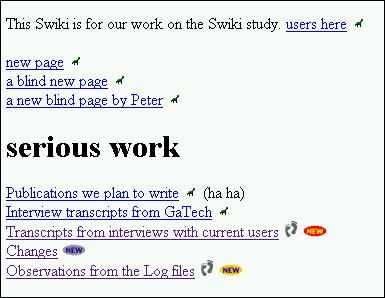
\includegraphics[width=\textwidth]{scrsh_coweb_contextual}
      \caption[CoWeb Contextual Cues]{%
      CoWeb Contextual Cues,
        retrieved January 25, 2008, from
        \url{http://homepage.mac.com/juggle5/WORK/publications/SwikiWriteup.html}.
      }
      \label{figure:scrsh.coweb.contextual}
    \end{minipage}
    \hfill
    \begin{minipage}[t]{0.475\wholewidth}
      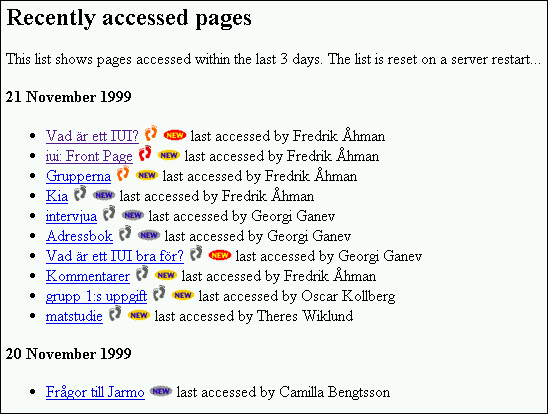
\includegraphics[width=\textwidth]{scrsh_coweb_global}
      \caption[CoWeb Global Cues]{%
      CoWeb Global Cues,
        retrieved January 25, 2008, from
        \url{http://homepage.mac.com/juggle5/WORK/publications/SwikiWriteup.html}.
      }
      \label{figure:scrsh.coweb.global}
    \end{minipage}
  \end{whole}
  \normalcaption
\end{figure}

We use \emph{social texture} to describe socially constructed annotations or
visualizations which may be used for navigation or in some form guide
users in navigational choices.

Social texture ties in with the forms of social navigation we've
recently discussed. Tagging for instance is a social texture.
The interaction history systems we've discussed uses forms of visualizations
in close proximity to hyperlinks to convey their degree of usage. This is also
a form of social texture.

The first forms of social texture used in computer systems to our knowledge is
\citet{hill92}'s usage of \emph{computational wear} which is an analogy for
the wear physical objects experience when used. They modify a text editor to
show both wear related to document edits and readings of documents. This wear
is graphically visualized trough the editor's scroll bar.
The concept of edit and read wear has since been used on the Web in for
instance the Footprints system \citep{wexelblat99}.

\citet{xu06} modified a Wiki with the aim of integrating social navigational
mechanisms. They used read-wear information for creating social
texture in the Wiki both inline pages, on a page level, and on a global
level. \citeauthor{xu06} took the approach of displaying read-wear in real
time, thus making the system a populated space. To make such an approach
usefull the Wiki needs a certain ammount of users present at all times. If
it's not frequently trafficed it would probably be better to represent
historical read-wear as done in CoWeb \citep[p.~220]{dieberger00a}. Both
contextual and global use of such social texture can be seen in
\figureref{scrsh.coweb.contextual} and \figureref{scrsh.coweb.global}.

``virtPresenter'' is a hypermedia based lecture viewer where read-wear have
been used to visualize a groups' interaction with continuous content
\citep{mertens06}. By following the traces other users have left current users
can interpret what's the most sought after parts of a lecture. The
visualization is implemented in ways similar to \citet{hill92} by showing
graphs of usage in line with a timeline selector and can be seen in
\figureref{scrsh.virtpresenter.timeline}.

\begin{figure}[b]
  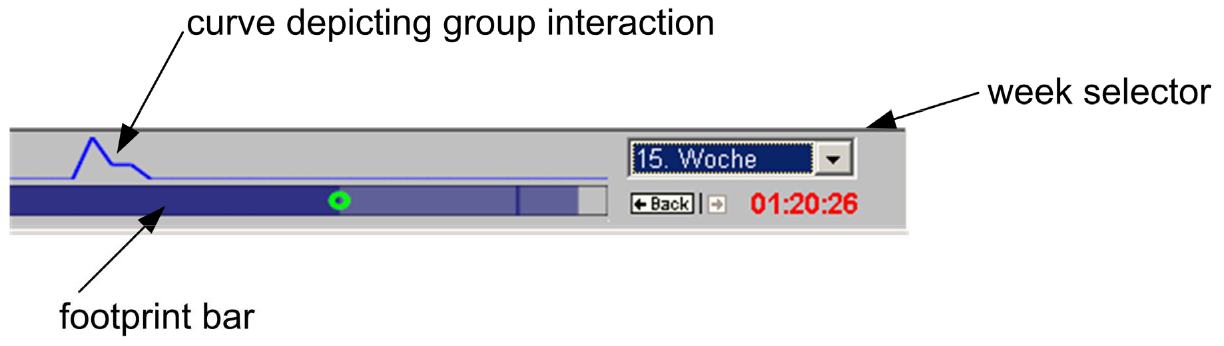
\includegraphics[width=0.9\textwidth]{scrsh_virtpresenter_timeline}
  \caption[virtPresenter Timeline]{
    virtPresenter Timeline \citep[p.~43]{mertens06}.
  }
  \label{figure:scrsh.virtpresenter.timeline}
\end{figure}


\subsubsection{Search}
% social search articles and semantic web/search article
% not that relevant as we're focusing on navigation trough browsing

We've noted that it was experienced that users potentially could become lost
or disorientated in hypertext even before the comming of the Web. It was known
that search could be a remedy for this problem:

\begin{citequote}[p.~38]{conklin87}
  One solution to this dilemma is to apply standard data\-base search and
  query techniques to locating the node or nodes which the user is seeking.
  This is usually done by using boolean operations to apply some combination
  of keyword search, full string search, and logical predicates on other
  attributes (such as author, time of creation, type, etc.) of nodes or links.
\end{citequote}

\subsection{Usefulness}
% dieberger00b:
%   filtering: HEE - find most relevant info
%              RecSys - pick items from a large space
%   quality:   HEE - find quality info (interesting, valid)
%   social affordance: HEE - users aware of each other
%                          - social experience
%                      - space is alive
%                        - not only affect navigation
%                          - stay longer in the space
%                          - relaxed
%                          - try new features

\citet{svensson05} performed a troughout evaluation of the Kalas system and
two issues in perspective of social navigation:
\begin{enumerate}
  \item Will social navigation enable users to navigate more efficiently?
  \item Do social navigation increase the perceived subjective quality of
    a navigation process?
\end{enumerate}

Server logs were statistically mined and more in depth qualitative interviews
were conducted. The results showed that people tended to move to the most
populated part of system and used recommendations for helping select which
items to navigate. \citeauthor{svensson05} also found that the subjects
overall had a positive impression of the social features of the system. They
seemed more interested in expressing themselves trough such features than
using information from others to help their navigation process.

Favorable results for the effectiveness of social navigation was found during
a simulation experiment conducted by \citeauthor{riedl03}. In most
circumstances social navigation resulted in superior performance contrasted
with asocial navigation. It's important to note that social navigation
decreased the effectiveness of navigation in some instances of their
simulations \citeyearpar[p.~365]{riedl03}.
Interestingly it was also discovered that social navigation was more
beneficial in environments with high uncertainty%
\sidenote{
  \citeauthor{riedl03} says that the two sources of such uncertainty is
    ``arising from the correctness of the information gained in any state,
    and the potential difficulty of reaching that state to obtain
    the information'' \citeyearpar[p.~363]{riedl03}.
}
than environments with higher certainty--provided that the
simulated users could reach the social media, the social texture
\citeyearpar[p.~368]{riedl03}. 

\section{Building on Top of the Web}
% Greasemonkey, hoodwink.d, new hoodwink.d service
% browser extensions related, Greasemonkey itself a extension, but
% thinking about specialized plugins for enabling interaction on top of other
% web pages.
% mashups kind of related, maybe put inside web2.0 part or separate part
% open apis is the fuel for mashups. possible without by screen scraping, but
% not as convenient and safe (upgrades on the pages we're scraping)
% facebook, open social. applications on top of social network sites. installed base
% of users and relationships already in place.

